%%%%%%%%%%%%%%%%%%%%%%%%%%%%%%%%%%%%%%%%%
% Dreuw & Deselaer's Poster
% LaTeX Template
% Version 1.0 (11/04/13)
%
% Created by:
% Philippe Dreuw and Thomas Deselaers
% http://www-i6.informatik.rwth-aachen.de/~dreuw/latexbeamerposter.php
%
% This template has been downloaded from:
% http://www.LaTeXTemplates.com
%
% License:
% CC BY-NC-SA 3.0 (http://creativecommons.org/licenses/by-nc-sa/3.0/)
%
%%%%%%%%%%%%%%%%%%%%%%%%%%%%%%%%%%%%%%%%%

%----------------------------------------------------------------------------------------
%	PACKAGES AND OTHER DOCUMENT CONFIGURATIONS
%----------------------------------------------------------------------------------------

\documentclass[final,hyperref={pdfpagelabels=false}]{beamer}

\usepackage[orientation=portrait,size=a0,scale=0.94]{beamerposter} % Use the beamerposter package for laying out the poster with a portrait orientation and an a0 paper size

\usetheme{I6pd2} % Use the I6pd2 theme supplied with this template

\usepackage[english]{babel} % English language/hyphenation

\usepackage{amsmath,amsthm,amssymb,latexsym} % For including math equations, theorems, symbols, etc

%\usepackage{times}\usefonttheme{professionalfonts}  % Uncomment to use Times as the main font
%\usefonttheme[onlymath]{serif} % Uncomment to use a Serif font within math environments

\usepackage{graphicx}
\usepackage{framed}
\usepackage{mathtools}
\DeclarePairedDelimiter{\floor}{\lfloor}{\rfloor}

\boldmath % Use bold for everything within the math environment

\usepackage{booktabs} % Top and bottom rules for tables

\graphicspath{{figures/}} % Location of the graphics files

\usecaptiontemplate{\small\structure{\insertcaptionname~\insertcaptionnumber: }\insertcaption} % A fix for figure numbering

%----------------------------------------------------------------------------------------
%	TITLE SECTION 
%----------------------------------------------------------------------------------------

\title{\huge Precise and Efficient Model-Based Vehicle Tracking Method Using
Rao-Blackwellized and Scaling Series Particle Filters} % Poster title

\author{Mengwen He$^{1^*,3^*}$, Eijiro Takeuchi$^{1,3}$, Yoshiki Ninomiy$^{2,3}$, and Shinpei Kato$^{3,4}$} % Author(s)

\institute{$^1$Graduate School of Information Science, Nagoya University (* left since April, 2016)\\
	$^2$Institute of Innovation for Future Society (MIRAI), Nagoya University\\
	$^3$JST/COI, Nagoya (* left since April, 2016)\\
	$^4$Graduate School of Information Science and Engineering, the University of Tokyo} % Institution(s)

%----------------------------------------------------------------------------------------
%	FOOTER TEXT
%----------------------------------------------------------------------------------------

\newcommand{\leftfoot}{http://www.coi.nagoya-u.ac.jp/} % Left footer text

\newcommand{\rightfoot}{mengwenh@andrew.cmu.edu} % Right footer text

%----------------------------------------------------------------------------------------

\begin{document}

\addtobeamertemplate{block end}{}{\vspace*{2ex}} % White space under blocks

\begin{frame}[t] % The whole poster is enclosed in one beamer frame

\begin{columns}[t] % The whole poster consists of two major columns, each of which can be subdivided further with a	nother \begin{columns} block - the [t] argument aligns each column's content to the top

\begin{column}{.02\textwidth}\end{column} % Empty spacer column

\begin{column}{0.47\textwidth} % The first column

%----------------------------------------------------------------------------------------
%	OBJECTIVES
%----------------------------------------------------------------------------------------

\begin{block}{Objective}

\begin{itemize}
\item Develop a precise and efficient high-dimensional particle filter (PF) based vehicle tracking method for the intelligent vehicle to interact with the surrounding vehicles on the road (Fig. \ref{fig:accident}).
\end{itemize}

\begin{figure}
	\centering
	\includegraphics[width=0.95\textwidth]{./img/accident}
	\caption{Precise and efficient tracking of a target vehicle can sensitively detect the driver's intension and will lead to reliable predictions for ensuring safe driving. For example: (Left) in the parking-lot, when a parked vehicle starts moving out, its small position change should be tracked for collision avoidance; (Middle) on the road, when a running vehicle tends to change lane, its small orientation change should be tracked for safe overtaking; (Right) at the intersection without traffic light, when a speedy vehicle comes out, its speed change should be tracked for deciding whether to pass the intersection.}
	\label{fig:accident}
\end{figure}

\end{block}

%----------------------------------------------------------------------------------------
%	INTRODUCTION
%----------------------------------------------------------------------------------------
            
\begin{block}{Introduction}

\begin{itemize}
\item Vehicle tracking technique enables the intelligent vehicle to interact with the surrounding vehicles (Fig. \ref{fig:accident}).
\item Bayesian approach is a common and efficient method to solve object-tracking problems.
\item PF is a type of non-parametric Bayesian filter:
\begin{itemize}
	\item Advantages: can represent complex beliefs and copes with non-linear motion models.
	\item Disadvantages: computational cost increases exponentially with the tracking state's dimensionality.
\end{itemize}
\item Rao-Blackwellized PF (RBPF) and Scaling Series PF (SSPF) can relief the curse of dimensionality:
\begin{itemize}
	\item RBPF: marginalize some parameters in the tracking state and use Gaussian estimate to track them.
	\item SSPF: annealing-based interactive PF focuses limited particles on the regions with higher probability.
\end{itemize}
\item This paper presents an improved vehicle tracking method by combining RBPF and SSPF (noted as RBSSPF).
\end{itemize}
\end{block}

\begin{block}{Contributions}

\begin{itemize}
	\item We introduced the latest measurement into the motion estimate to get accurate pose update. (FastSLAM 2.0)
	\item With the new tracking method, we fully exploited the advantage of SSPF through the entire tracking process.
	\begin{itemize}
		\item Motion: SSPF directly estimates the next pose using non-linear motion models with the latest measurement.
		\item Geometry: SSPF derives the best geometry fitting results even with a partial observation (multi-mode problem).
	\end{itemize}
	\item We conducted an experiment using two intelligent vehicles to evaluate our tracking method:
	\begin{itemize}
		\item Both vehicles use Velodyne and 3D point cloud map to derive accurate localization results as ground-truth.
		\item 10 km driving distance of public dataset with flat roads, narrow streets, and steep ramps.
	\end{itemize}
\end{itemize}

\end{block}

%----------------------------------------------------------------------------------------
%	METHODS
%----------------------------------------------------------------------------------------

\begin{block}{General Tracking Method Description}

\begin{center}
\textbf{(1) The Dynamic Bayesian Network (DBN) of Our Tracking Method}
\end{center}
\begin{columns}[t]
	\begin{column}{0.48\textwidth}
		\begin{figure}
			\centering
			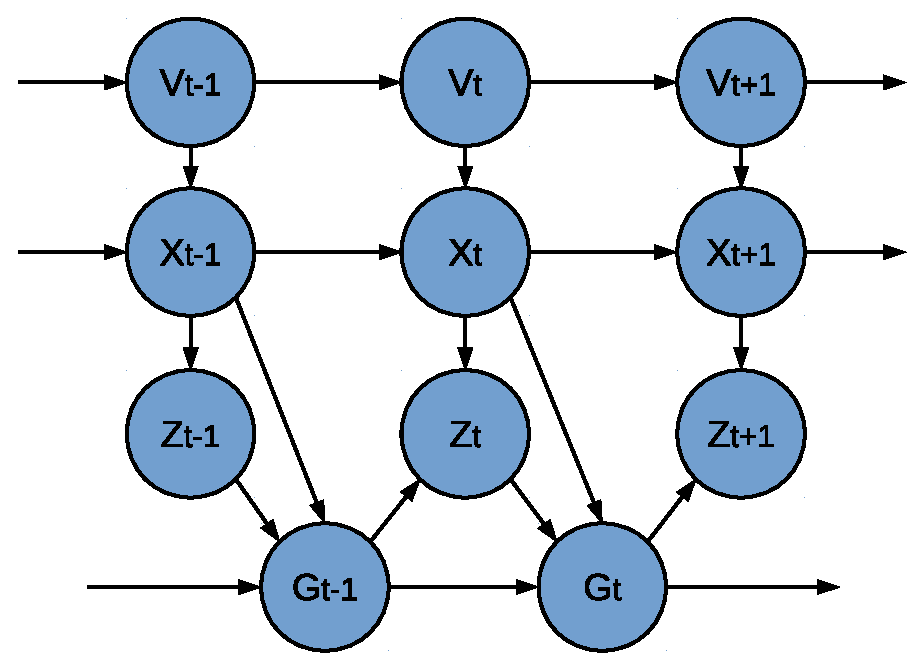
\includegraphics[width=0.95\textwidth]{./img/DBN}
			\caption{The modified DBN in our tracking method, which introduces the latest measurement into the motion estimate. The representation of this DBN is that for a target target vehicle and a given sensor measurement $Z_t$ at time $t$, we estimate the vehicle's pose $X_t$, motion $V_t$, and geometry $G_t$.}
			\label{fig:DBN}
		\end{figure}
	\end{column}
	
	\begin{column}{0.48\textwidth}
			\begin{center}
				\textbf{The Update Equations of The DBN in Fig. \ref{fig:DBN}}
			\end{center}
			\begin{itemize}
				\item Upper part: motion estimate:
				\begin{itemize}
					\item Motion model:~
					$\left\{\begin{array}{l}
					p(V_t|V_{t-1}) \\
					p(X_t|X_{t-1},V_t)
					\end{array}\right.$
					\item Measurement model:~
					$p(Z_t|X_t,G_{t-1})$
					\begin{itemize}
						\item The estimate of $V_t$ and $X_t$ considers $Z_t$.
						\item $Z_t$ is related to the true geometry $G^{**}$.
						\item Both $G^{**}$ and $G_t$ are still unknown.
						\item But $G_t$ will converge to constant $G^{**}$.
						\item We use $G_{t-1}$ for the motion estimate at $t$.
					\end{itemize}
				\end{itemize}
				\item Lower part: geometry estimate:
				\begin{itemize}
					\item Geometry update:~
					$p(G_t|X_t,G_{t-1},Z_t)$
				\end{itemize}
				\item The Bayesian belief at time $t$ according to the history of the estimate of the pose, motion, and geometry based on a set of sensor measurement:
				$$Bel_t=p(X^t,V^t,G^t|Z^t)$$
			\end{itemize}			
	\end{column}
\end{columns}

\vspace{1em}
\begin{center}
\textbf{(2) The Solution of The Bayesian Belief $Bel_t$}
\end{center}
$$Bel_t = p(G_t|X^t,V^t,G^{t-1},Z^t) \cdot p(X_t,V_t|X^{t-1},V^{t-1},G^{t-1},Z^t) \cdot p(X^{t-1},V^{t-1},G^{t-1}|Z^t) = S_t \cdot R_t \cdot Bel_{t-1}$$
\vspace{-2em}
\begin{columns}[t]
	\begin{column}{0.48\textwidth}
		\begin{center}
			\textbf{Step 1: Motion Estimate}
		\end{center}
		\begin{itemize}
			\item The motion Posterior $R_t$:
			\begin{equation}
				\small
				\nonumber
				\begin{array}{rcl}
				  R_t & = & p(X^{t-1},V^{t-1},G^{t-1}|Z^t) \\
				  	  & \propto & p(Z_t,X_t,V_t|X^{t-1},V^{t-1},G^{t-1},Z^{t-1}) \\
			      & = & p(Z_t|X^t,V^t,G^{t-1},Z^{t-1}) \\
			      &   & \cdot p(X_t|X^{t-1},V^t,G^{t-1},Z^{t-1}) \\
			      &   & \cdot p(V_t|X^{t-1},V^{t-1},G^{t-1},Z^{t-1}) \\
			      & = & p(Z_t|X_t,G_{t-1}) \cdot p(X_t|X_{t-1},V_t) \cdot p(V_t|V_{t-1}) \\
			      & \propto & p(X_t,V_t|X_{t-1},V_{t-1},G_{t-1},Z_t)
			 	\end{array}
			\end{equation}
			\item We can use the SSPF (an optimization method) to directly optimize $R_t$ based on $X_{t-1}$, $V_{t-1}$, $G_{t-1}$, and $Z_t$. Then we can get the updated motion $V_t$ and pose $X_t$.
			\item The SSPF optimization for the motion estimate is similar to the scan-matching in FastSLAM 2.0.
		\end{itemize}		
	\end{column}
	\begin{column}{0.48\textwidth}
		\begin{center}
			\textbf{Step 2: Geometry Estimate}
		\end{center}
		\begin{itemize}
			\item The geometry posterior $S_t$ conditioned on motion:
			\begin{equation}
			\small
			\nonumber
			 \begin{array}{rcl}
			  S_t & = & p(G_t|X^t,V^t,G^{t-1},Z^t) \\
			      & \propto & p(Z_t,G_{t-1},X_t,G_t|X^{t-1},V^t,G^{t-2},Z^{t-1}) \\
			      & = & p(Z_t|X^t,V^t,G^t,Z^{t-1}) \\
			      &   & \cdot p(G_{t-1}|X^t,V^t,G_t,G^{t-2},Z^{t-1}) \\
			      &   & \cdot p(X_t|X^{t-1},V^t,G_t,G^{t-2},Z^{t-1}) \\
			      &   & \cdot p(G_t|X^{t-1},V^t,G^{t-2},Z^{t-1}) \\
			      & \propto & p(Z_t|X_t,G_{t-1}) \cdot S_{t-1}
			 \end{array}
			\end{equation}
			\item $G_{t-1}$ is out of date after the motion estimate.
			\item Replace $p(Z_t|X_t,G_{t-1})$ with the measurement likelihood $p(Z_t|X_t,G)$ to obtain better geometry estimate $G^*$ from geometry fitting done by SSPF.
			\item Linearize $p(Z_t|X_t,G)$ on $G$ in Gaussian form $\mathcal{N}(G^*,\sigma)$ to perform RBPF on $G_t$ estimate:
			$$S_t \propto p(Z_t|X_t,G) \cdot S_{t-1} \sim \mathcal{N}(G^*,\sigma) \cdot S_{t-1}$$
		\end{itemize}
	\end{column}
\end{columns}

\vspace{1em}
\begin{center}
\textbf{(3) The Method Framework}
\end{center}
\begin{columns}[t]
	\begin{column}{0.48\textwidth}
		\begin{figure}
			\centering
			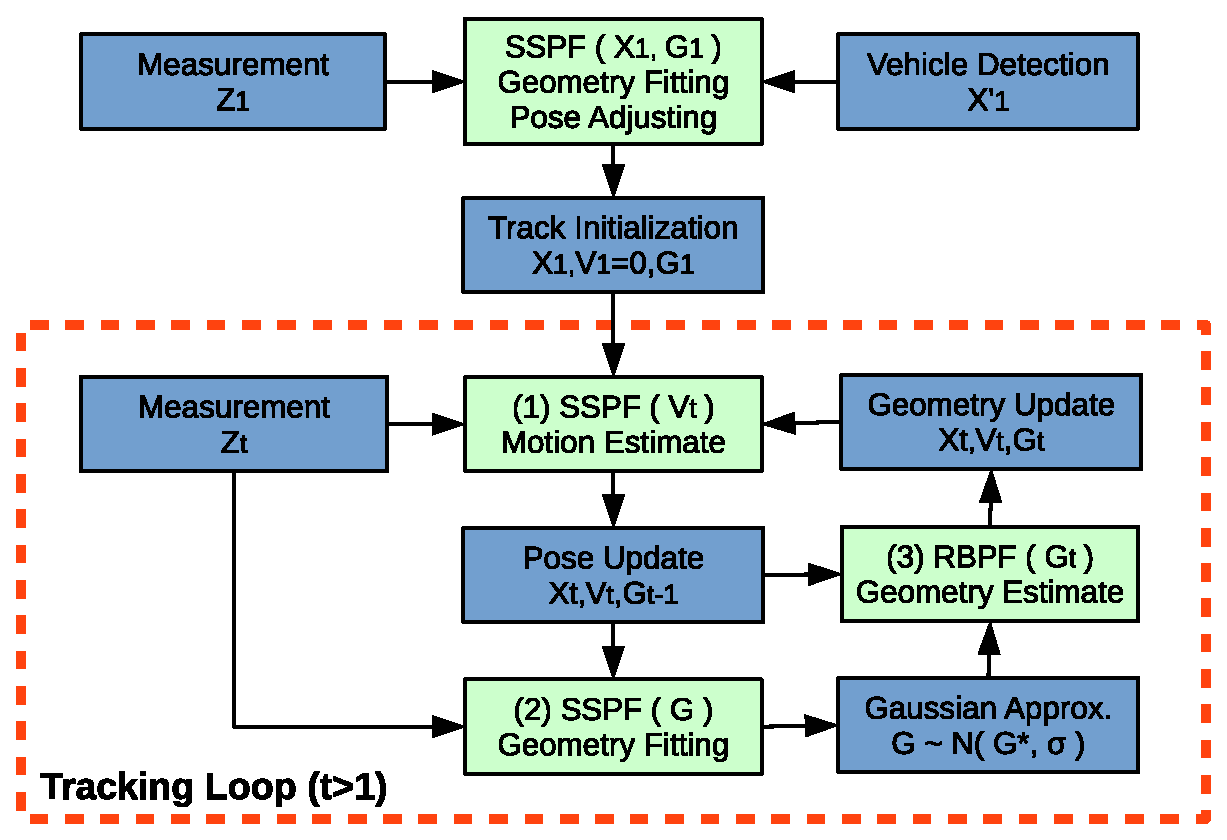
\includegraphics[width=\textwidth]{./img/framework}
			%\caption{The framework of our tracking method.}
			\label{fig:framework}
		\end{figure}
	\end{column}
	\begin{column}{0.48\textwidth}
		\begin{center}eps
		\textbf{Summary of The General Tracking Method}
		\end{center}
		\begin{itemize}
		\item Bayesian belief of tracking and update equation
		\begin{itemize}
		\item $Bel_t=p(X^t,V^t,G^t|Z^t)$
		\item $Bel_t=S_t \cdot R_t \cdot Bel_{t-1}$
		\end{itemize}
		\item Motion estimate and pose update ($X_t$ and $V_t$)
		\begin{itemize}
		\item SSPF on $R_t\propto p(X_t,V_t|X_{t-1},V_{t-1},G_{t-1},Z_t)$
		\end{itemize}
		\item Geometry fitting and linearization ($p(Z_t|X_t,G)$)
		\begin{itemize}
		\item SSPF on $p(Z_t|X_t,G)$ with respect to $G$ $\Rightarrow G^*$
		\item $p(G|X_t,Z_t) \sim \mathcal{N}(G^*,\sigma)$ (Laplace approx.)
		\end{itemize}
		\item Geometry estimate ($G_t$)
		\begin{itemize}
		\item RBPF on $S_t \propto N(G^*,\sigma) \cdot S_{t-1}$
		\end{itemize}
		\end{itemize}
	\end{column}
\end{columns}


\end{block}

%----------------------------------------------------------------------------------------

\end{column} % End of the first column

\begin{column}{.02\textwidth}\end{column} % Empty spacer column
 
\begin{column}{.48\textwidth} % The second column


%----------------------------------------------------------------------------------------
%	Algorithm SECTION
%----------------------------------------------------------------------------------------

\begin{block}{Tracking Method Implementation}
\begin{center}
\textbf{(1) Tracking State Definition \& Ackerman-Steering Motion Model}
\end{center}
\begin{columns}[t]
	\begin{column}{0.48\textwidth}
	\begin{itemize}
	\item Our tracking implementation works on a 2D coordinates with 10 dimensional state:
	\end{itemize}
		\begin{table}
			\centering
			%\caption{Notation of State's Parameters in Our Implementation \label{tab:notation}}
			\begin{tabular}{|c|c|c|}
			\hline
			             & \bf{Parameters} & \bf{Note} \\
			\hline
			             & $x,y$ & position of anchor point\\
			\cline{2-3}
			Pose ($X$)   & $\theta$ & orientation of vehicle \\
			\hline
			             & $\alpha^*$ & orientation offset of velocity \\
			\cline{2-3}             
			             & $v$ & velocity \\
			\cline{2-3}
			Motion ($V$) & $\kappa$ & curvature \\
			\hline
			             & $wl,wr$  & distance to left/right edge \\
			\cline{2-3}
			Geometry ($G$) & $lf,lb$  & distance to front/back edge \\
			\hline
			\end{tabular}
			\end{table}
	* Because the anchor point is randomly selected from the detection result (Fig.\ref{fig:framework} upper) and the geometry is temporarily unknown, the variable $\alpha$ adjusts the velocity direction to be tangential to the circular trajectory (Fig.\ref{fig:geometry_ackerman}).
	\end{column}
	\begin{column}{0.48\textwidth}
	\begin{figure}
	 \centering
	 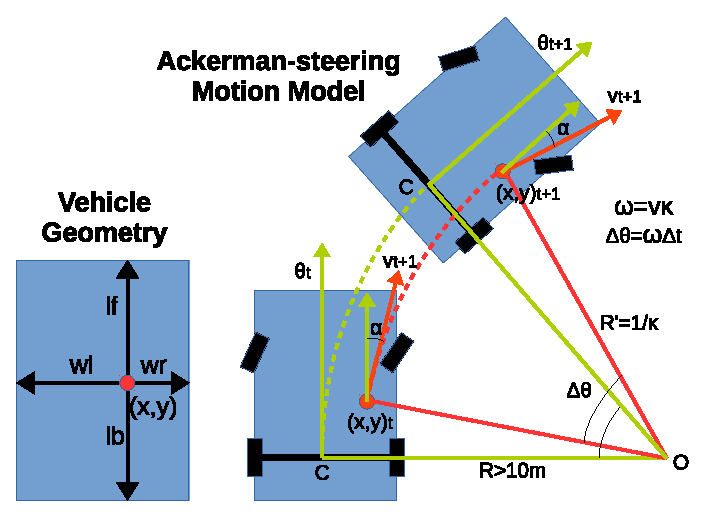
\includegraphics[width=\textwidth]{./img/geometry_ackerman}
	 %\caption{The illustration of vehicle's geometry and motion model.}
	 \label{fig:geometry_ackerman}
	\end{figure}
	\end{column}
\end{columns}

\vspace{1em}
\begin{center}
\textbf{(2) Virtual Scan \& Measurement Model}
\end{center}
\begin{columns}[t]
	\begin{column}{0.53\textwidth}
		\begin{itemize}
			\item We developed a noval virtual scan algorithm to convert the 3D Velodyne point cloud to a 2D scan range array. (published on IV16: \textit{``Robust Virtual Scan for Obstacle Detection in Urban Environments"})
			\item The measurement model and the cost function are shown as right figure. $d_{min}$--$A$ corresponds to the occlusion area, $A$--$B$ corresponds to the free space, $B$--$D$ corresponds to the vehicle's surface, and $D$--$d_{max}$ corresponds to the passing through the vehicle.
			\item The measurement model is used by the SSPF, which gives best results for continuous and differentiable beliefs with varying gradients; therefore, the common constant cost function is approximated by exponential functions.
			
		\end{itemize}
	\end{column}
	\begin{column}{0.43\textwidth}
		\begin{figure}
		 \centering
		 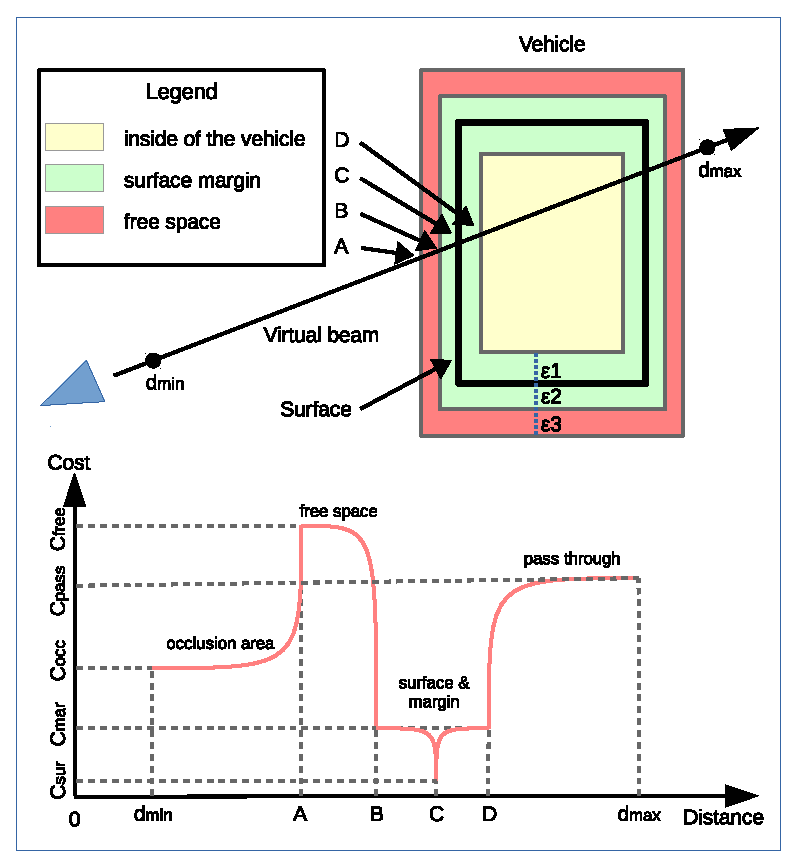
\includegraphics[width=0.8\textwidth]{./img/measure.eps}
		 %\caption{The illustration of vehicle's measurement model and the continuous cost function.  \label{fig:measure}}
		\end{figure}
	\end{column}
\end{columns}
\end{block}


%----------------------------------------------------------------------------------------
%	Experiment RESULTS
%----------------------------------------------------------------------------------------

\begin{block}{Experiment Results}

\vspace{-2em}
\begin{columns}[t]
	\begin{column}{0.48\textwidth}
		\begin{center}
			\textbf{Platforms \& Driving/Tracking Trajectories}
		\end{center}
		\begin{figure}
		 \centering
		 \includegraphics[width=0.8\textwidth]{./img/matsu.eps}\\
		 \vspace{1em}
		 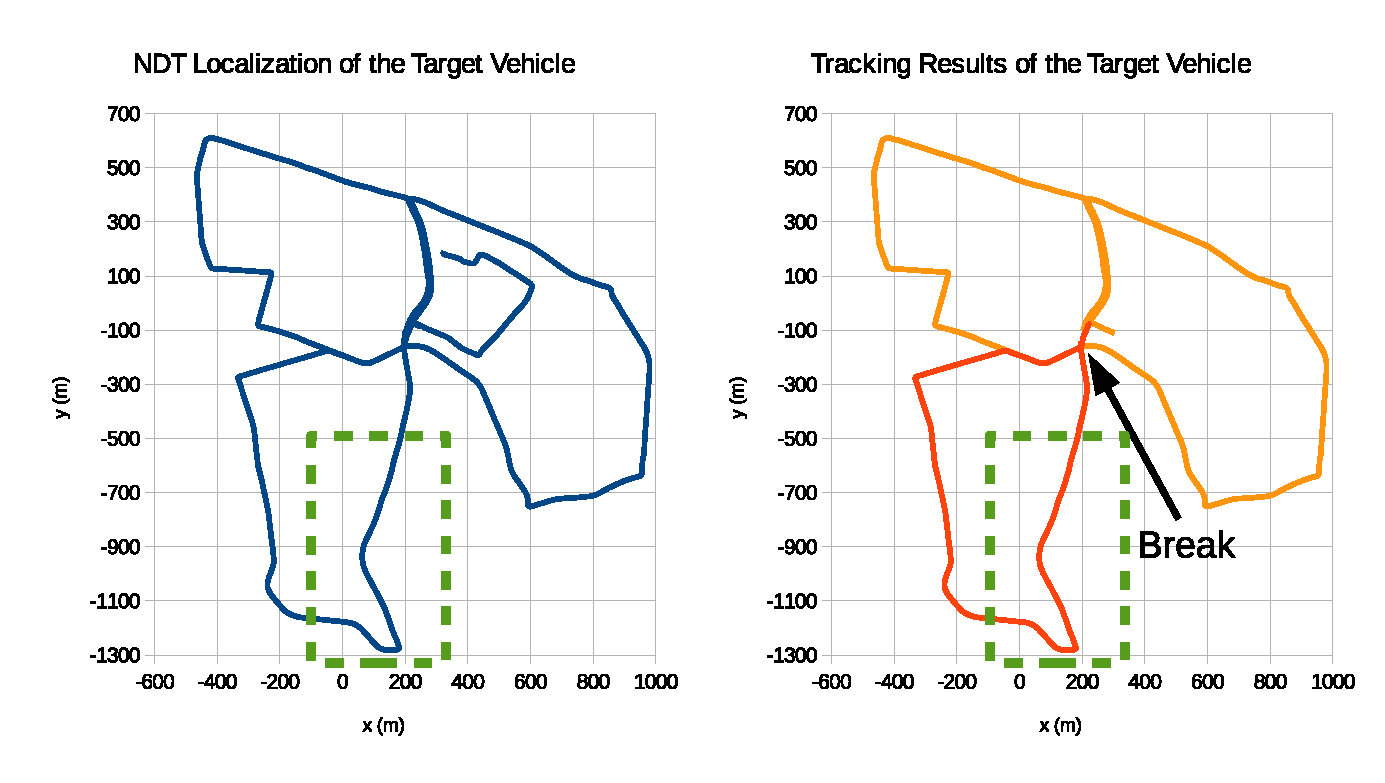
\includegraphics[width=0.9\textwidth]{./img/path.eps}
		 \caption{The target vehicle "ZMP Silver" and the ego-vehicle "Matsu". The green rectangle is the "challenge" area for evaluation. \label{fig:matsu}}
		\end{figure}
	\end{column}
	\begin{column}{0.48\textwidth}
		\begin{center}
			\textbf{The Particle Number of RBSSPF}
		\end{center}
		\begin{figure}u
		 \centering
		 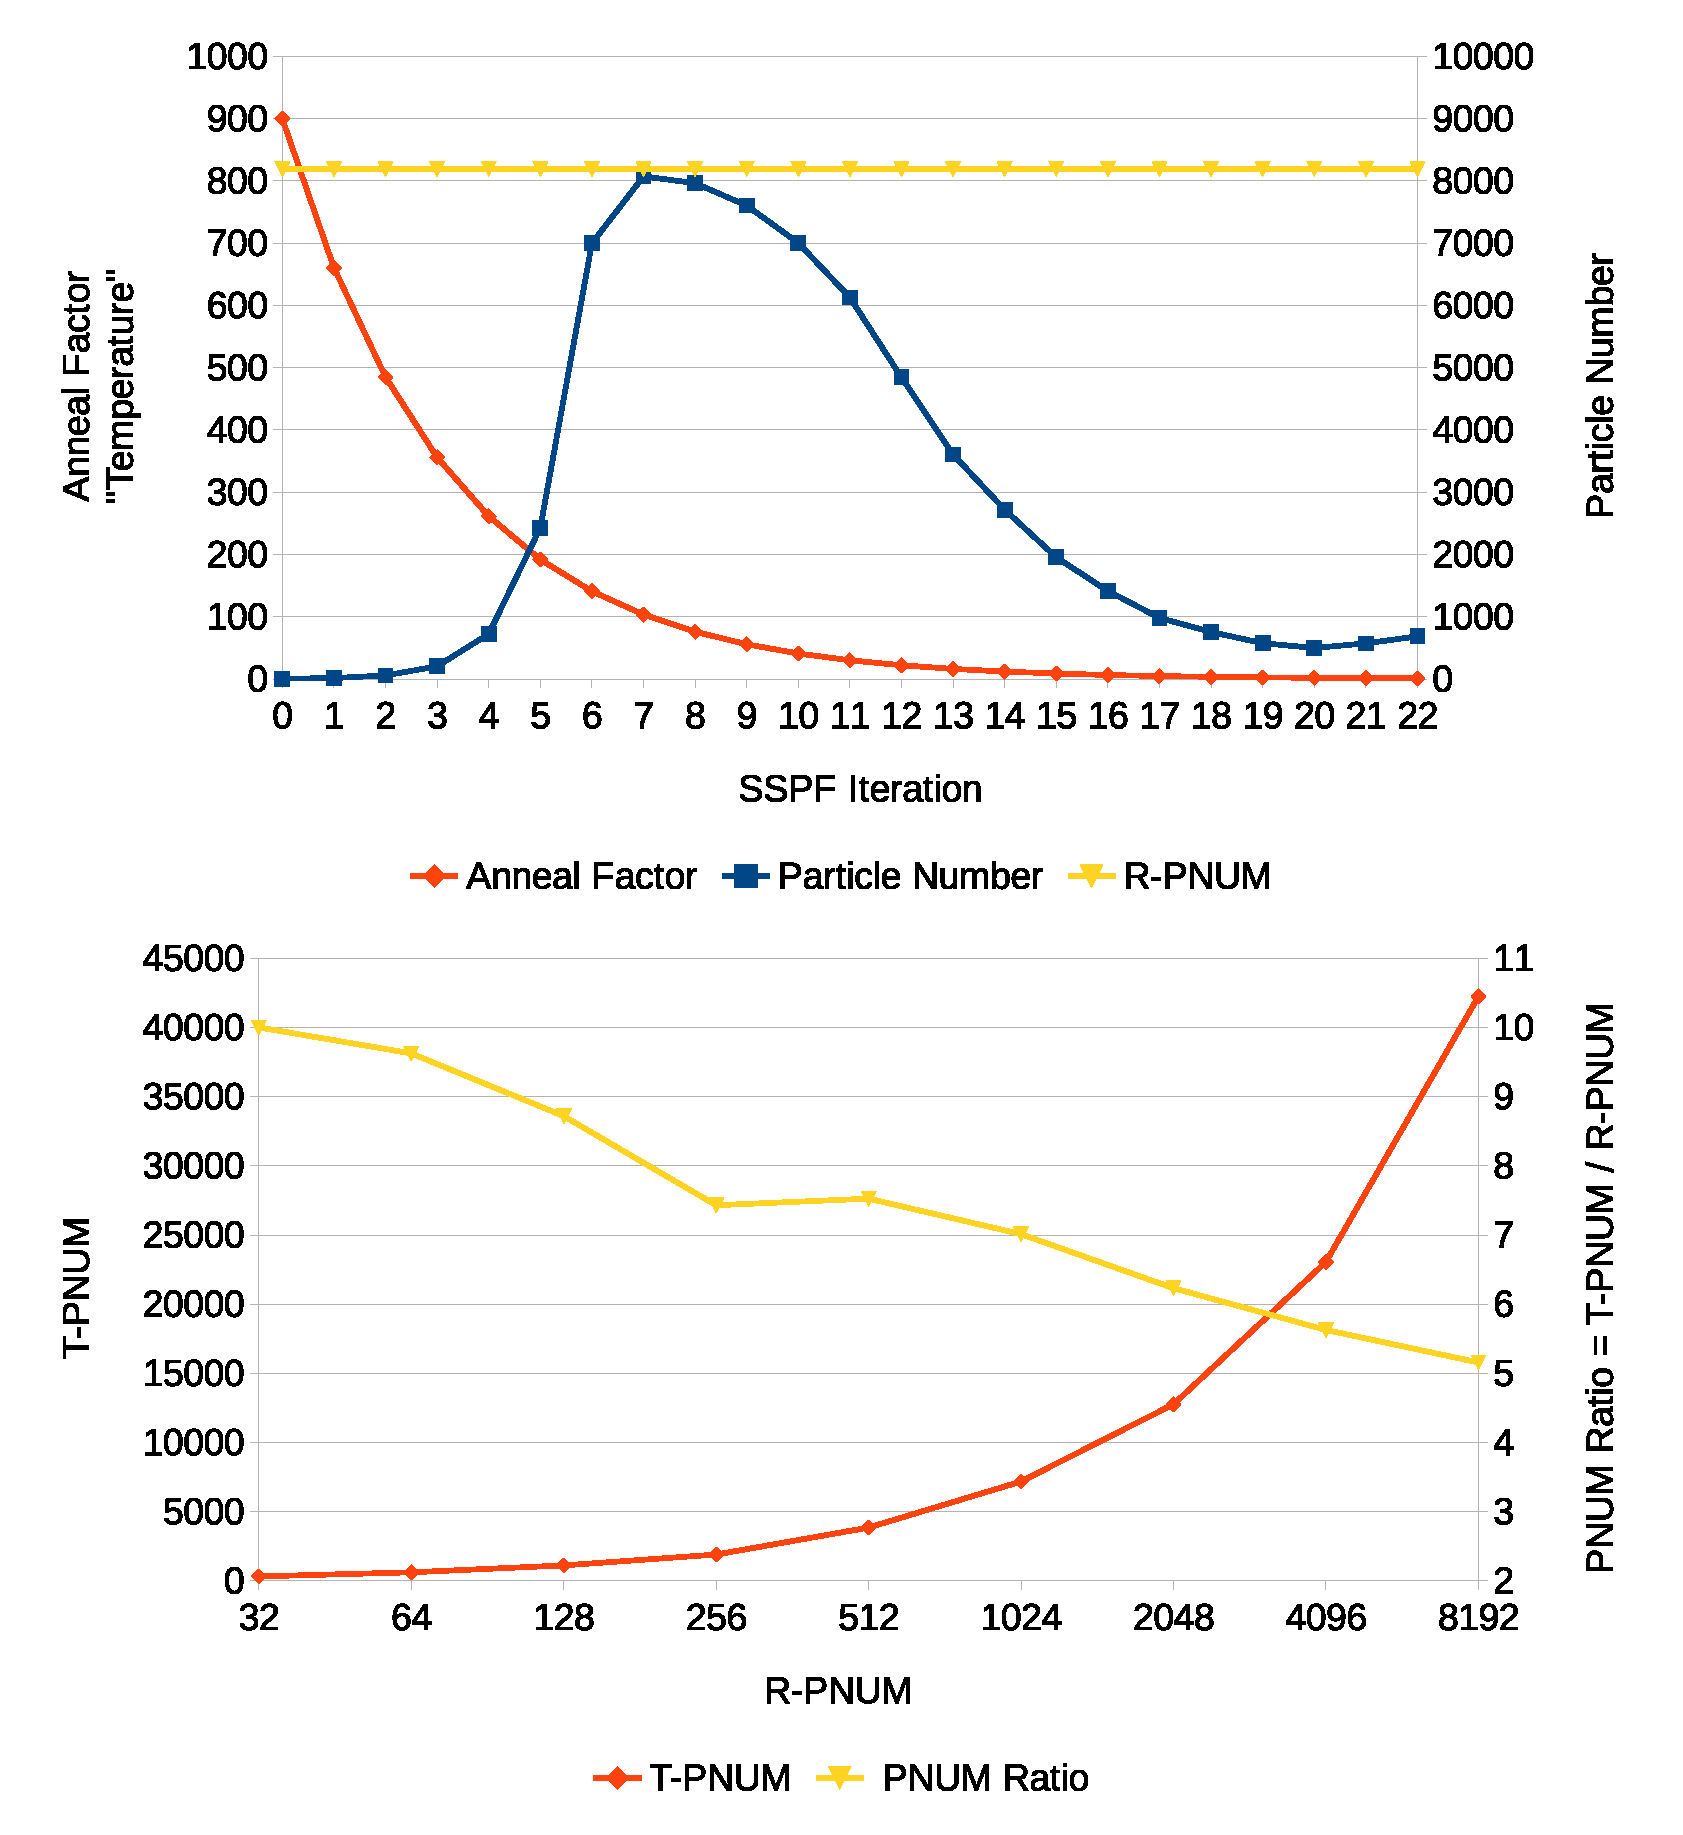
\includegraphics[width=0.8\textwidth]{./img/SSPF-Iteration}
		 \caption{R-PNUM: required number of particles after each resampling. T-PNUM: total number of particles after all iterations. \label{fig:SSPF-Iteration}}
		\end{figure}
	\end{column}
\end{columns}
\vspace{1em}
\begin{center}
\textbf{The Evaluation and Comparison with RBPF Tracking Results (In The Green Rectangle Area)}
\end{center}
\begin{itemize}
\small
\item Orange: ground-truth; Blue: RBPF; Red: RBSSPF.
\item Left: One example of the tracking results (RBPF: R-PNUM=2048; RBSSPF: R-PNUM=64).
\item Right: The comparison of RMSE vs. CPU computational time (T-PNUM) between RBPF and RBSSPF.
\end{itemize}
\begin{columns}[t]
\begin{column}{0.18\textwidth}
\begin{figure}
 \centering
  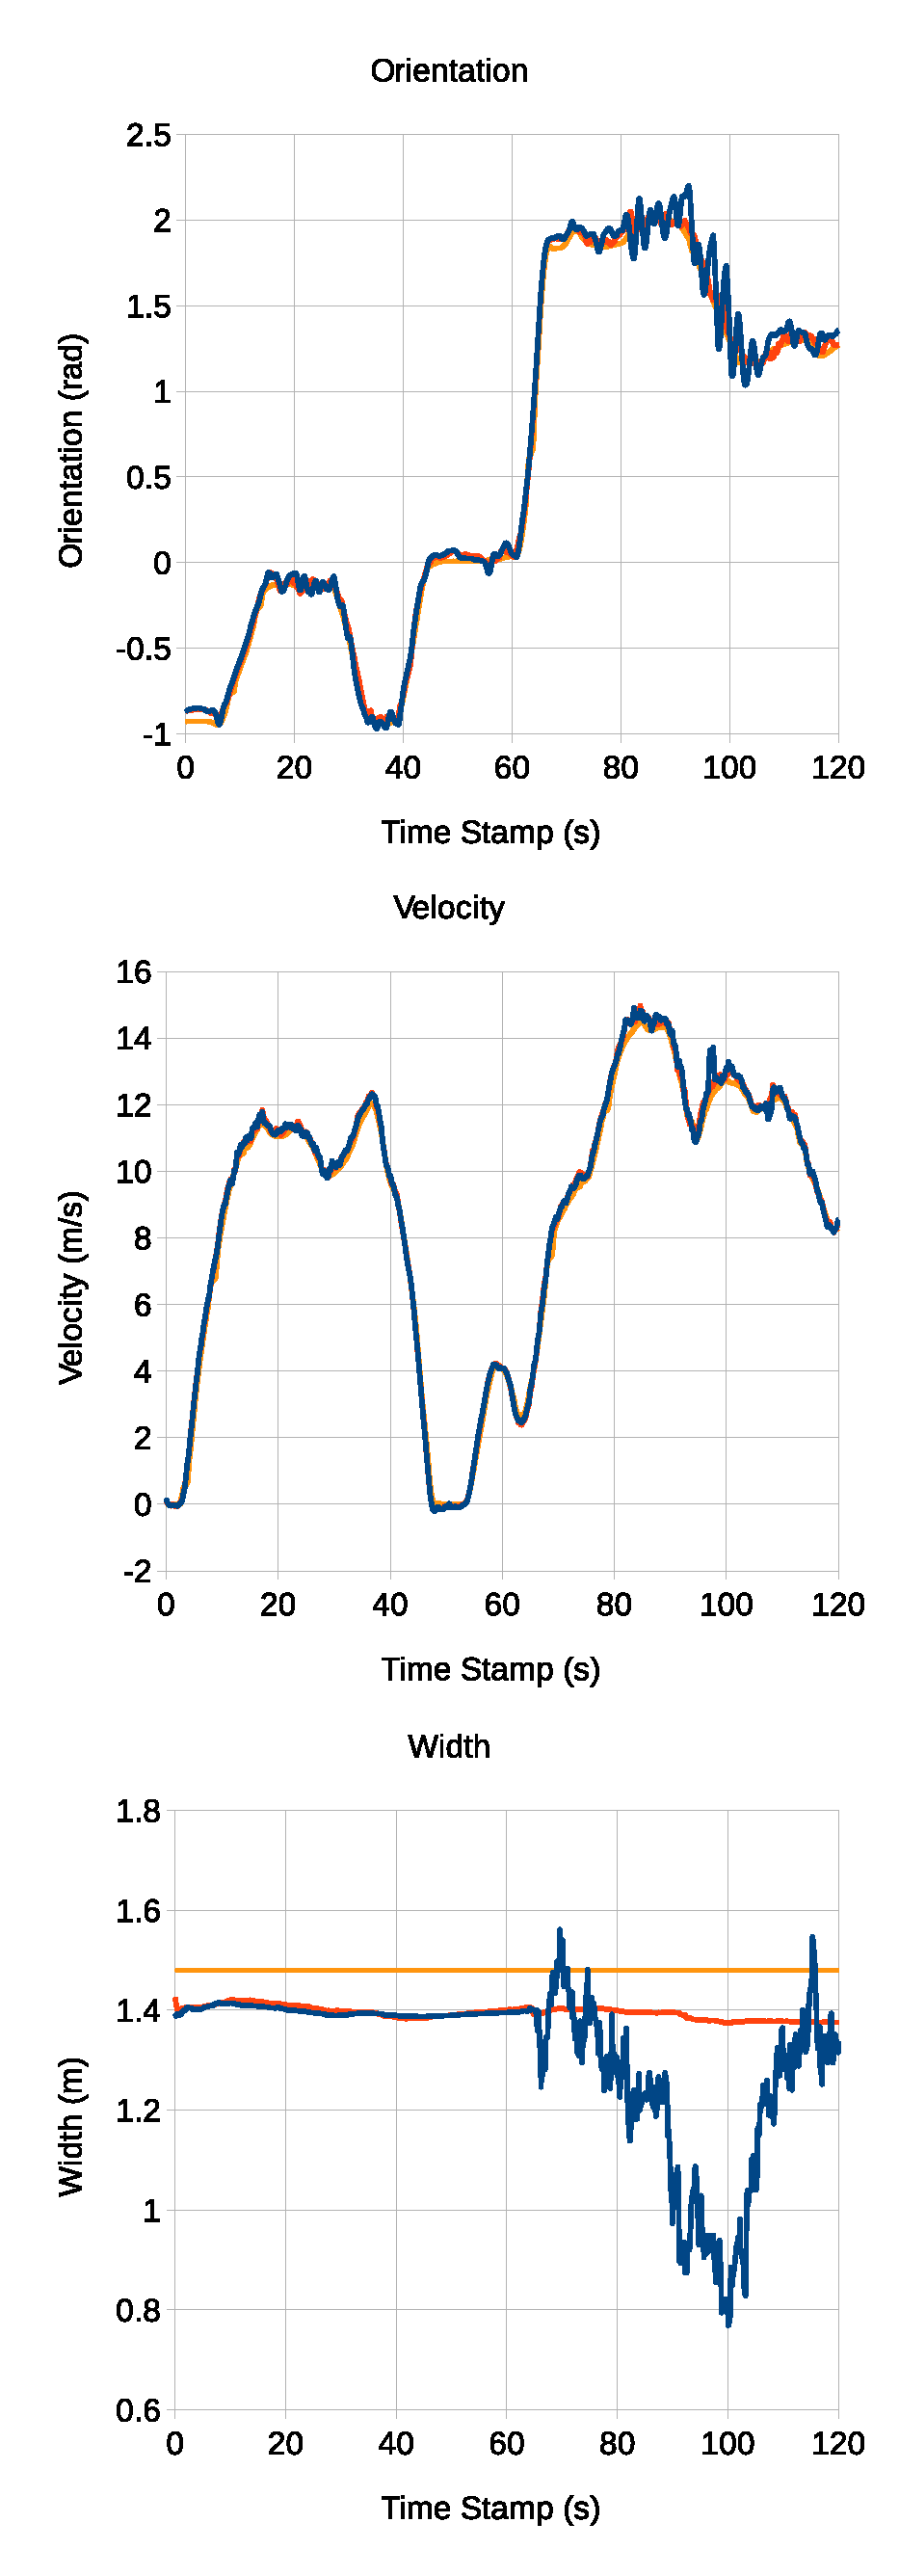
\includegraphics[width=1\textwidth]{./img/ground-truth.eps}
\end{figure}
\end{column}
\begin{column}{0.8\textwidth}
\begin{figure}
 \centering
 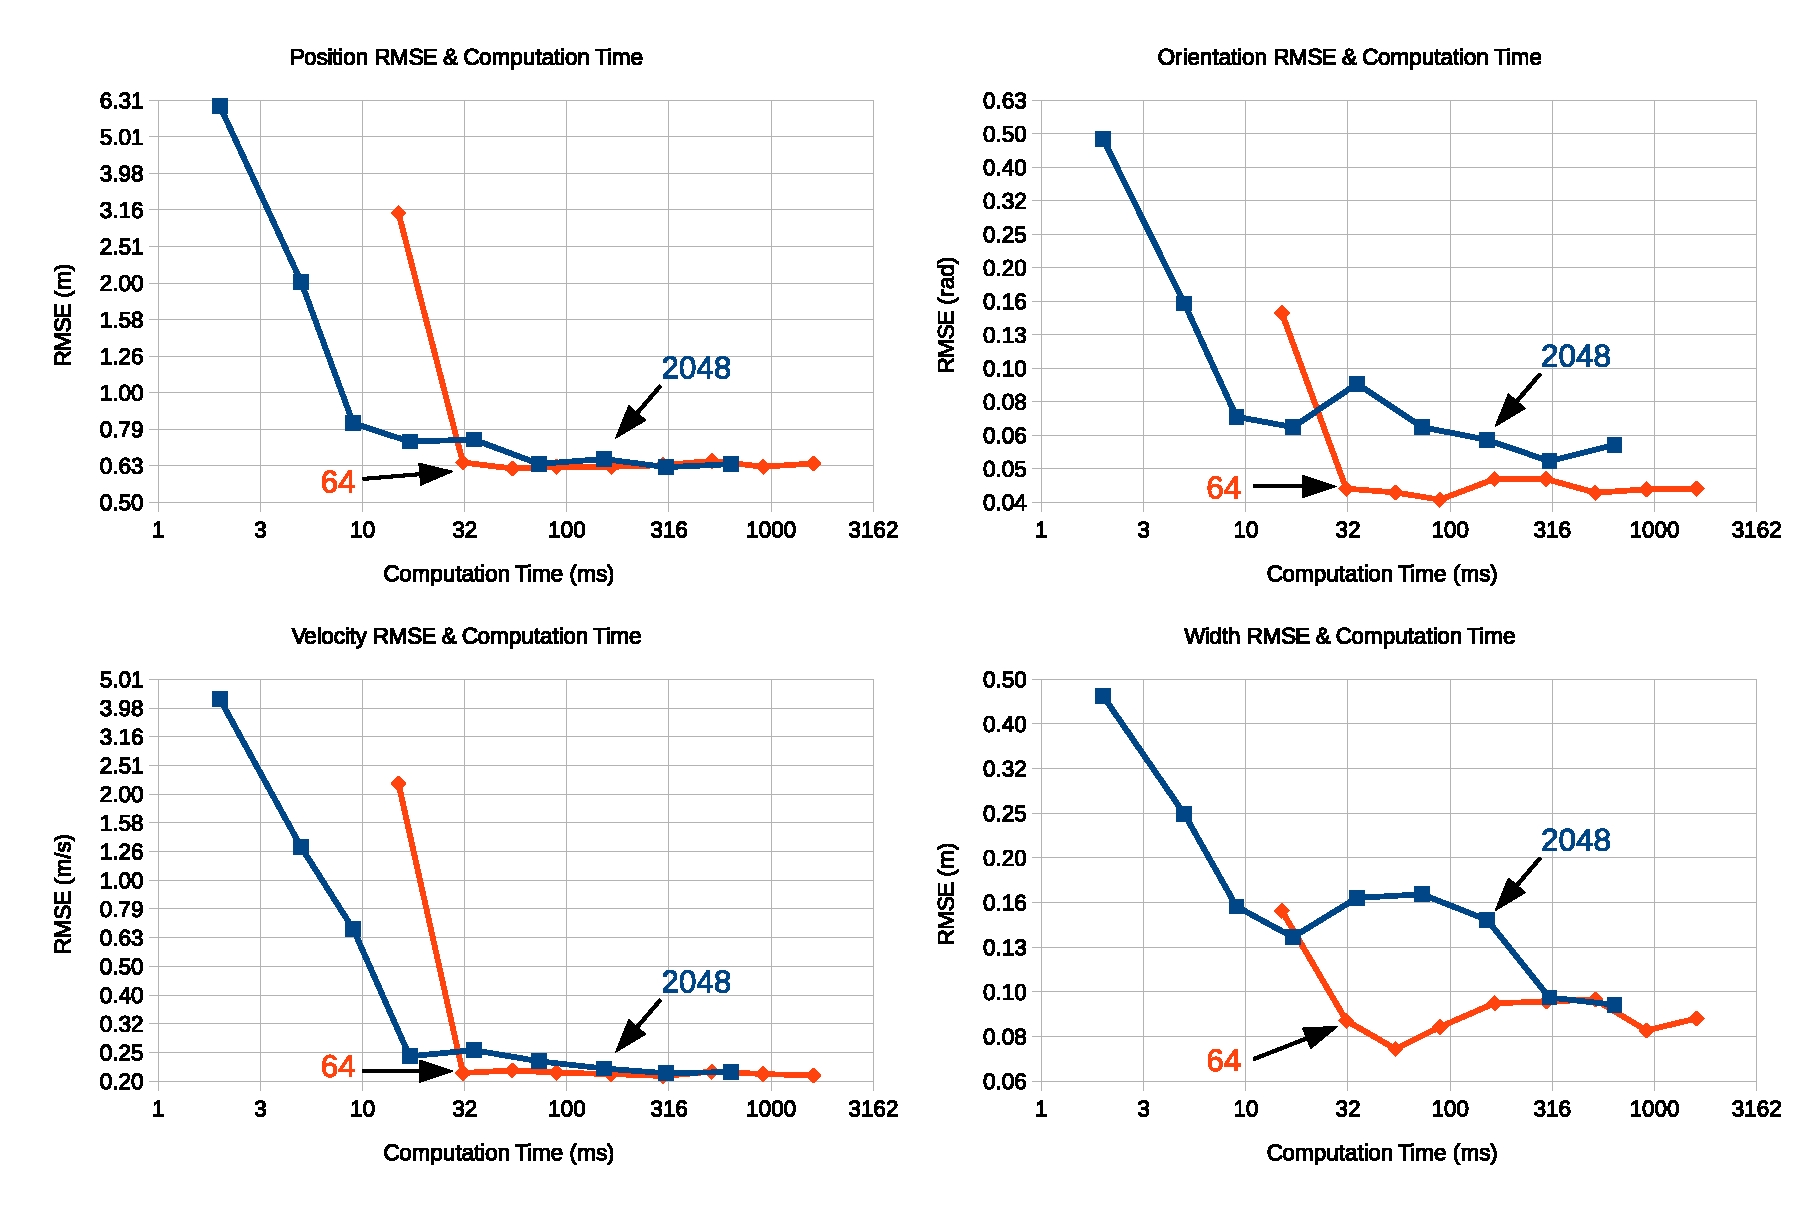
\includegraphics[width=1\textwidth]{./img/rmse.eps}
\end{figure}
\end{column}
\end{columns}

\vspace{1em}
\begin{columns}[c]
\begin{column}{0.4\textwidth}
The conclusion of evaluation results:
\begin{itemize}
	\item The minimum RMSE of the RBSSPF is not greater than that of the RBPF, and specifically, the RBSSPF is more precise in orientation and width estimate than RBPF.
	\item The RBSSPF spends less iime (R-PNUM=64) to achieve the level of minimum RMSE than the RBPF (R-PNUM$\geq$1024).
	\item If we constrain the computation time of tracking, the RBSSPF can obtain more precise results than RBPF, and if we require to	reach a certain level of accuracy, the RBSSPF spends less time than the RBPF.
	
	 		
\end{itemize}
\end{column}
\begin{column}{0.55\textwidth}
\begin{framed}
\begin{center}
\textbf{The GPU Acceleration for Real-time Tracking}
\end{center}
\begin{figure}
 \centering
 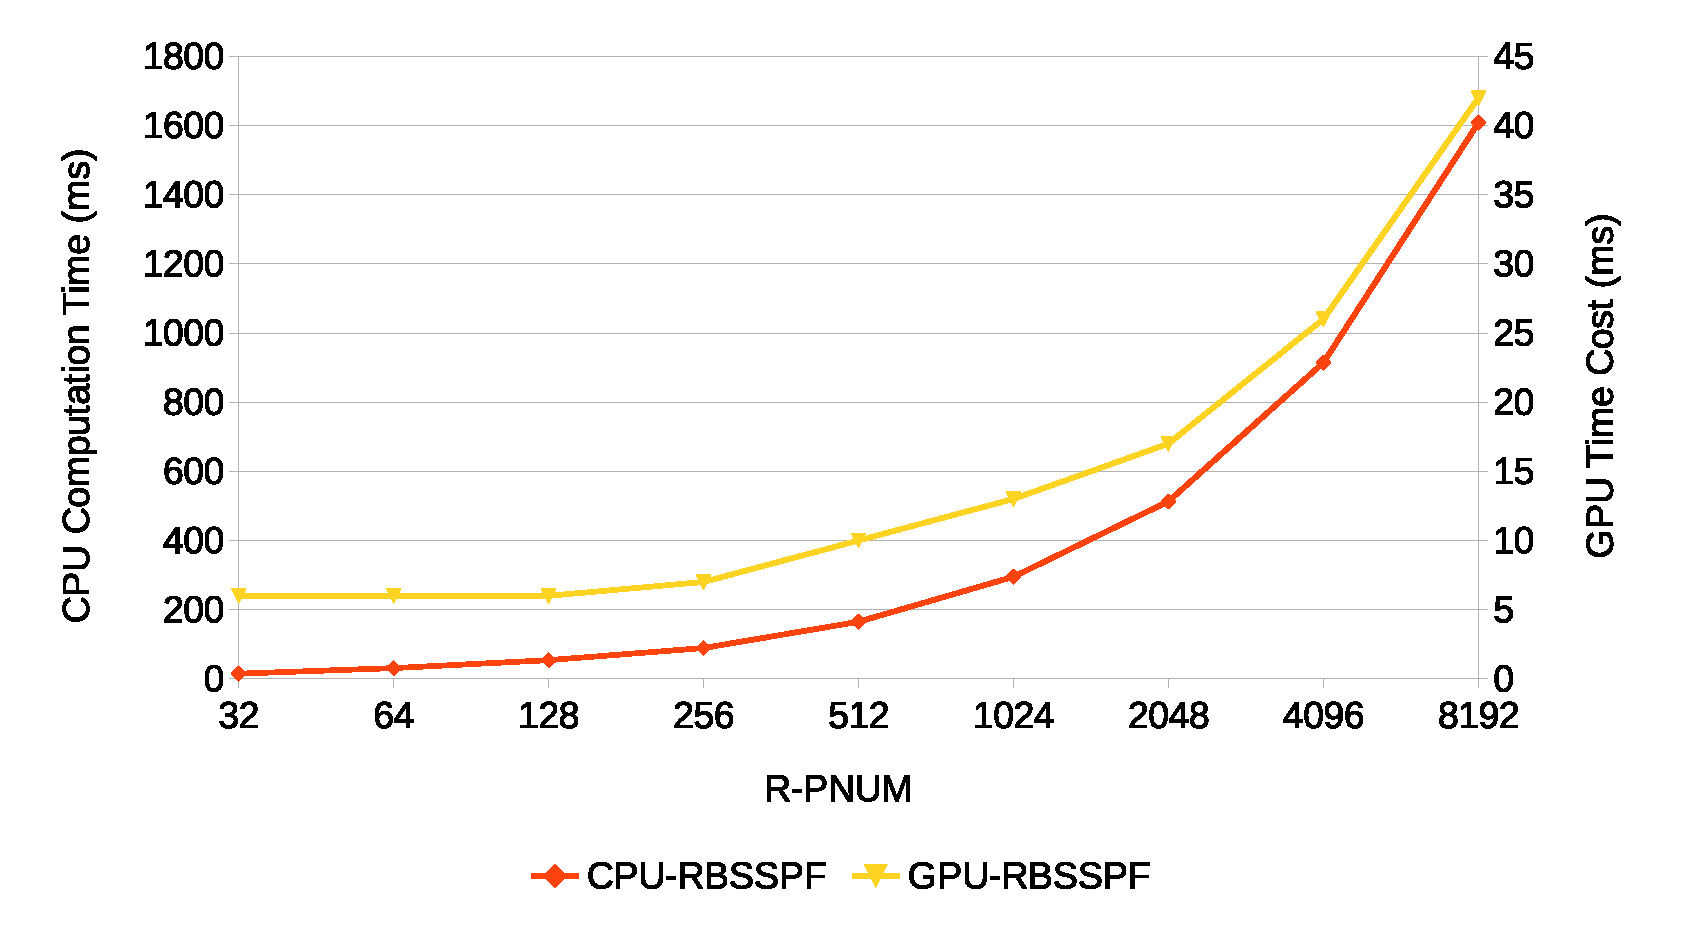
\includegraphics[width=0.85\textwidth]{./img/time.eps}
\end{figure}
\end{framed}
\end{column}
\end{columns}


\end{block}

%----------------------------------------------------------------------------------------

\end{column} % End of the second column

\begin{column}{.015\textwidth}\end{column} % Empty spacer column

\end{columns} % End of all the columns in the poster

\end{frame} % End of the enclosing frame

\end{document}